\documentclass[10pt,a4paper]{article}
\usepackage[T1]{fontenc}
\usepackage[utf8]{inputenc}
\usepackage[english]{babel}
\usepackage{lmodern}
\usepackage{microtype}
\usepackage[a4paper,margin=1.8cm]{geometry}
\usepackage{amsmath,amssymb}
\usepackage{booktabs}
\usepackage{graphicx}
\usepackage[font=small]{caption}
\usepackage{enumitem}
\usepackage[hidelinks]{hyperref}
\usepackage{natbib}
\setcitestyle{authoryear,round,aysep={,},yysep={;}}
\graphicspath{{figures/}}
\setlength{\parskip}{0.22em}
\setlength{\parindent}{0pt}

\title{What Binarization Costs Virtual Screening Encoders
\thanks{Code and per-target metrics:
\url{https://github.com/josefslink/binary-hashing-virtual-screening}}}
\author{Josef Scheifinger}
\date{September 2026}

\begin{document}
\maketitle

\begin{abstract}
Virtual screening at a billion-molecule scale is limited less by encoders than by the cost
of storing and comparing their output, which is why binary hash codes have become a promising
representation. DrugHash proposes learning those codes during training and reports that this
is necessary, but it publishes neither code nor weights. This report reproduces two
structure-aware virtual screening models, SPRINT and DrugCLIP, on LIT-PCBA and DUD-E and then
measures what binarizing their embeddings produces. Both reproductions land within one to two
points of their published AUROC, though DrugCLIP's DUD-E BEDROC comes back 3.2 points low. Against this baseline, two findings were discovered. The
two encoders respond to binarization in opposite directions, across 117 SPRINT and 115 DrugCLIP
targets: subtracting a shared per-dimension reference before binarizing lifts DrugCLIP above its
own baseline by 0.019 AUROC but costs SPRINT 0.28 to 0.30, and even the per-type reference that
suits SPRINT best still costs it 0.06 to 0.12. The reason is visible in their per-dimension
statistics rather than in the method. Furthermore, post-hoc
binarization and a trained hashing objective preserve different halves of the ranking -
centering recovers global ranking quality while losing early enrichment and a hash head
trained on frozen encoders does the inverse, improving BEDROC by 14\% and EF 0.5\% by 13.6\%
while AUROC moves only 2.2\%. Because DrugHash's own $\lambda = 0$ ablation binarized without
any centering step, its reported advantage over not hashing is an upper bound on what its
training contributes.
\end{abstract}

\section{Story Summary}\label{sec:story}

\begin{enumerate}[leftmargin=*]
\item \textbf{What is the central question?}\\
What does binarizing a virtual screening model's embeddings actually cost in retrieval
quality and does training a hashing objective into the model achieve something that
binarizing a finished model cannot?

\item \textbf{Why is this question important?}\\
Screening libraries contain billions of compounds, so storing one embedding per molecule at
32 bits per dimension runs into terabytes, whereas one bit per dimension would reduce that by
a factor of 32. DrugHash reports that a hashing objective has to be trained into the model
for this to work, but since neither code nor weights have been published, the claim cannot be
easily verified.

\item \textbf{What evidence/data are needed to answer this question?}\\
A fair reproduction of both models as a baseline, post-hoc binarization measured across
several centering schemes on both benchmarks (LIT-PCBA and DUD-E) and several code lengths,
and the same objective applied during training so that the two routes are directly
comparable.

\item \textbf{What methods are used to get this evidence/data?}\\
The released checkpoints of SPRINT and DrugCLIP were run on LIT-PCBA and DUD-E with the
encoder outputs captured, without the published code being modified. Five centering schemes
and five code lengths were then applied to the cached embeddings and a $128 \rightarrow 128$
dimensional L2-normalised head was trained on frozen DrugCLIP encoders under DrugHash's
objective across a $\lambda$ grid, where $\lambda$ weights the hashing term in the loss.

\item \textbf{What analyses must be applied to the data?}\\
AUROC, BEDROC and enrichment factors per target, averaged over targets, together with paired
per-target comparisons so that a mean is not driven by a few outliers. Additionally the
per-dimension distribution statistics of both encoders were computed to explain why they
differ, and the benchmark actives were compared against the list of molecules the released
DrugCLIP checkpoint was trained on, in order to measure how much of its benchmark performance
could be memorisation rather than retrieval.

\item \textbf{What evidence/data were obtained?}\\
Both models were reproduced within one or two points on AUROC, and on BEDROC everywhere except
DrugCLIP on DUD-E, which is 3.2 points low. The
two encoders produced opposite orderings of the centering schemes, identically on both
benchmarks, and the trained hashing head improved BEDROC by 14\% and EF 0.5\% by 13.6\% while
AUROC increased only 2.2\%.

\item \textbf{What were the results of the analyses?}\\
Subtracting one shared per-dimension reference from both the molecule and the pocket
embeddings before binarizing improves global ranking by 0.019 AUROC while lowering BEDROC by
0.027, and the trained hashing objective does the inverse. The difference between the two
models is linked to their per-dimension distributions, where DrugCLIP's mean sits at the
49.9th percentile of its own dimension and SPRINT's at the 96.7th.

\item \textbf{How did the analyses answer the central question?}\\
Binarization costs early enrichment rather than global ranking and a trained objective
addresses exactly the part that post-hoc binarization loses. Because DrugHash's own
$\lambda = 0$ ablation binarized without any centering step, its measured advantage over not
hashing is an upper bound on what the training contributes.

\item \textbf{What does this answer tell us about the broader field?}\\
A hashing scheme developed on one encoder cannot be assumed to transfer to another, since the
effect depends on the geometry of the embedding space rather than on the method alone.
Furthermore, compression methods for screening should be judged on early-recognition metrics
rather than AUROC.
\end{enumerate}

\section{Introduction}\label{sec:intro}

Drug discovery is expensive and slow, and virtual screening addresses part of that by ranking
molecules computationally before the most promising candidates are tested in a wet-lab. Modern
screening libraries are measured in billions of compounds, which means the ranking step has to
touch every entry in the library.

\subsection{Screening as retrieval}
Contrastive dual-encoder methods such as DrugCLIP \citep{bib:drugclip} and SPRINT
\citep{bib:sprint} made that step cheap. Both encode
protein pockets and molecules into a shared embedding space, so that screening reduces to a
similarity search and the expensive encoder runs once per molecule, rather than once per
screening task. This is what enables zero-shot screening at a scale traditional docking-based
methods cannot reach.

\subsection{The memory bottleneck}
What remains expensive is the library itself. Storing one billion molecules at SPRINT's 1024
dimensions in float32 requires roughly 4\,TB and even DrugCLIP's 128 dimensions require
roughly 0.5\,TB. This is the motivation for binary codes: one bit per dimension instead of 32
is a 32x reduction and Hamming distance reduces the retrieval to an XOR operation followed by
a population count, which is computationally very cheap. DrugHash \citep{bib:drughash} takes exactly this route,
adding a squared-error hashing loss to DrugCLIP's objective so that the encoder outputs
survive being binarized.

\subsection{The gap}
DrugHash reports that this training is necessary and supports that with an ablation in which
$\lambda$, the weight on the hashing term, is set to 0. That means no hashing during training
but $\operatorname{sign}(\cdot)$ still applied at evaluation. Their conclusion is that
accuracy then drops by a large margin. However, that ablation applies
$\operatorname{sign}(\cdot)$ directly to the raw embeddings, without first subtracting any
reference value, and it is therefore not obvious what a properly configured post-hoc
binarization would achieve. Because neither code nor weights were published, there is also no
reference implementation against which the claim could be checked.

\subsection{Objectives}
This report addresses three questions:
\begin{enumerate}[leftmargin=*]
\item Do the published LIT-PCBA \citep{bib:litpcba} and DUD-E \citep{bib:dude} numbers reproduce from the released checkpoints of
DrugCLIP and SPRINT?
\item What does post-hoc binarization of a frozen encoder cost, across centering schemes and
code lengths?
\item What does a trained hashing objective add on top of that?
\end{enumerate}

Both models were reproduced on both benchmarks, binarization was applied over cached
embeddings and a hash head was trained on frozen encoders under DrugHash's own objective.

\section{Background}\label{sec:background}

\subsection{The three methods}
\textbf{DrugCLIP} \citep{bib:drugclip} treats virtual screening as a cross-modal retrieval problem. Two Uni-Mol
\citep{bib:unimol} encoders, one for protein pockets and one for molecules, are trained contrastively so that a
pocket and its true binding partner end up close in a shared 128-dimensional embedding space.
At screening time the molecule library is encoded once offline, the query pocket is encoded
online and candidates are ranked by cosine similarity.

\textbf{SPRINT} \citep{bib:sprint} pursues the same retrieval formulation but is built for scale. Its molecule
side uses fingerprint features and its protein side uses SaProt \citep{bib:saprot}, a protein language model
whose vocabulary pairs each amino acid with a structural token. Its embeddings are
1024-dimensional, which is eight times DrugCLIP's and is the reason its memory footprint is
the larger of the two.

\textbf{DrugHash} \citep{bib:drughash} keeps DrugCLIP's encoders, training data and contrastive objective entirely
unchanged and adds one thing: a squared-error hashing loss that pulls each encoder output
towards its own sign pattern, so that the embeddings can be replaced by 128-bit codes and
retrieval by Hamming distance. Its novelty is therefore the objective and the retrieval space,
not the architecture.

\textbf{Uni-Core} \citep{bib:unicore} is not a model but the framework Uni-Mol and DrugCLIP are built on:
DrugCLIP's task definitions, data pipeline and evaluation entry points are registered through
it, so it must be installed for DrugCLIP to run.

\subsection{Metrics}
Both models rank candidates by the dot product of L2-normalised embeddings and where a target
has several pockets the maximum over them is taken.

Three metrics are reported throughout and the distinction between them matters, because the
key finding is that they move in different directions. AUROC is the probability that a
randomly chosen active is ranked above a randomly chosen inactive, which makes it global: a
method can improve it substantially without changing the first 0.5\% of the ranking at all.
BEDROC \citep{bib:bedroc} weights early ranks exponentially and is bounded in $[0,1]$. The enrichment factor at
0.5\% states how many times more actives appear in the top 0.5\% than in a random selection,
and is closest to what a screening task requires, since only a very small fraction of
candidates is ever tested experimentally.

BEDROC has a parameter $\alpha$ that sets how steeply early ranks are weighted, and the two
two models are evaluated at different values: SPRINT uses $\alpha = 85.0$, while DrugCLIP's
evaluation code hardcodes $\alpha = 80.5$ even though its paper reports BEDROC$_{85}$. I kept
each model's own value rather than picking one, because those are the values that reproduce
the published tables. The consequence is that BEDROC may be compared between my SPRINT rows
and SPRINT's paper, or between my DrugCLIP rows and DrugCLIP's paper, but a SPRINT BEDROC
should not be compared directly against a DrugCLIP BEDROC.

\subsection{DrugHash's objective}
DrugHash's objective is
\begin{equation}
L = L_c + \lambda \cdot L_{\text{hash}},
\end{equation}
where $L_c$ is DrugCLIP's inherited contrastive loss and $L_{\text{hash}}$ penalises the
squared distance between each encoder output and its own sign pattern, with the binary code
treated as a constant during the encoder update. The published optimal settings are
$\lambda = 0.2$ and 128-bit codes \citep{bib:drughash}.

\subsection{Benchmarks}
Two benchmarks are used. LIT-PCBA \citep{bib:litpcba} contains 15 targets with experimentally confirmed actives
and is the harder of the two - both models sit only slightly above chance. DUD-E \citep{bib:dude} contains 102
targets with property-matched decoys, is easier, and is the benchmark on which DrugHash's
published advantage over DrugCLIP is largest.

\section{Methods}\label{sec:methods}

\subsection{Setup, hardware and compute}
All experiments were run on a single workstation with a consumer GPU: an NVIDIA RTX 2070 with
8.1\,GB of VRAM, an AMD Ryzen 5 3600 with 12 threads and 15\,GB of system memory. The
pre-trained encoders of SPRINT and DrugCLIP were never fine-tuned and were only ever run in
inference mode, because end-to-end training of either model does not fit into 8\,GB. The only
component that was trained is the small hash head described in Section~\ref{sec:hash-head-method}, which has roughly
16.5k parameters per modality and 33k in total, and operates on embeddings that have already been computed, so it
trains on cached arrays rather than on the encoders themselves.

\begin{table}[h]
\centering
\small
\caption{\label{tab:runtimes}Approximate runtimes on the hardware above. The dumps write the encoder outputs to
disk once; everything in the results section is then computed from those files.}
\begin{tabular}{llr}
\toprule
Step & Benchmark & Runtime \\
\midrule
SPRINT full pass & LIT-PCBA & $\sim$15 min \\
SPRINT full pass & DUD-E & $\sim$30 min (first), $\sim$17 min after \\
DrugCLIP embedding dump & LIT-PCBA & $\sim$45 min \\
DrugCLIP embedding dump & DUD-E & $\sim$30 min \\
Hash head training & per $\lambda$ value & 2--3 min \\
Re-scoring one condition & either & $\sim$10 s \\
\bottomrule
\end{tabular}
\end{table}

Including runs repeated after bugs were found, the experiments took an estimated 15 to 20
GPU-hours.

The last row of Table~\ref{tab:runtimes} is what made the rest of the report possible on this hardware. Testing
six centering schemes on two models and two benchmarks would otherwise mean 24 full passes of
15 to 45 minutes each. Instead the encoder outputs are written to disk once per model and
benchmark, and every later experiment only changes how those stored arrays are scored. The
encoders are frozen, so the embeddings never change and this gives exactly the numbers a
re-run would - at about 10 seconds per condition instead of half an hour.

SPRINT and DrugCLIP have incompatible dependency stacks, so each runs in its own virtual
environment.

\subsection{Working with the published code without modifying it}
The copies of the SPRINT, DrugCLIP and Uni-Core repositories are unmodified and every change
this project requires is applied from outside at run time.

DrugCLIP's evaluation pipeline computes the embeddings, uses them and returns four summary
numbers, discarding the embeddings and the labels. That is sufficient for printing its AUROC,
but the goal was to use those embeddings. I implemented forward hooks on the two projection
heads to capture the embeddings while the upstream loop runs untouched, and the molecule
dataset's collater is wrapped to record the labels in batch order. The resulting arrays are
verified rather than assumed correct: on DUD-E the upstream routine does return its own score
vector, and recomputing that vector from the captured arrays reproduces it with a maximum
deviation of 0.0 on all 100 targets.

\subsection{Binarization and centering}
Binarizing an embedding means replacing each dimension with a single bit, according to whether
its value lies above or below some reference. For a drug matrix $D$ and a target matrix $T$
the code is $B = \mathbb{1}[X - r \geq 0]$ and similarity becomes $1 - d_H/d$, where $d_H$ is
the Hamming distance and $d$ the number of bits.

The choice of reference $r$ is the whole question. Five choices were swept, shown in Table~\ref{tab:modes}.
Two of them use the mean and two use the median, so both statistics were tested rather than
only one.

\begin{table}[h]
\centering
\small
\caption{\label{tab:modes}The five centering modes. \emph{Scope} is what the reference is computed over and
\emph{statistic} is how it is computed. \texttt{per\_type} and \texttt{global} are the
mean-based variants.}
\begin{tabular}{lll}
\toprule
Mode & Scope of the reference & Statistic \\
\midrule
\texttt{none} & none, threshold at zero & - \\
\texttt{per\_type} & separately per matrix, per dimension & mean \\
\texttt{per\_type\_median} & separately per matrix, per dimension & median \\
\texttt{global} & shared over $[D;T]$, per dimension & mean \\
\texttt{global\_median} & shared over $[D;T]$, per dimension & median \\
\bottomrule
\end{tabular}
\end{table}

The reason for testing both scopes is that they make opposite assumptions. A \emph{shared}
reference subtracts the same vector from molecules and pockets, which keeps them in the same
coordinate system - the two encoders were trained to align in that system, so preserving it
should help. A \emph{per-type} reference lets each side be centered on its own distribution,
which is the better estimate whenever a side has enough rows to compute a reliable statistic
from, but it moves the two sides independently and therefore risks breaking the alignment.

The median variants exist because the threshold is $\geq 0$, so a bit is balanced, meaning
roughly half the molecules get a 1, only if the reference splits that dimension in half. The
mean achieves this only for a symmetric distribution, whereas the median achieves it for any.
Whether balance actually helps is answered in Section~\ref{sec:why-differ}.

One case needs further mentioning, because it also produces plausible numbers. Centering a
one-row matrix by its own statistic yields exactly zero, so thresholding at $\geq 0$ produces
an all-ones code, which carries no information and drops that target out of its own evaluation
without raising an error. This affects FEN1 and OPRK1 on LIT-PCBA and every DUD-E target,
since all of them have a single pocket. Such matrices are left uncentered and a warning is
raised, so \texttt{per\_type} on DUD-E centers only the molecule side. This is a property of
the per-type scope rather than a fixable bug - a single row contains no distribution to
estimate from - and it is why \texttt{global}, whose reference comes from the concatenation of
both matrices, is the more meaningful comparison on DUD-E.

\subsection{Code length}
A $d$-dimensional embedding yields a $d$-bit code, so deciding how few bits a model needs is a
question about dimensionality. Three reductions were compared:
\begin{enumerate}[leftmargin=*]
\item Gaussian random projection followed by a sign, which is the standard
locality-sensitive hashing construction for cosine similarity \citep{bib:charikar} within the
general framework of \citet{bib:lsh}, seeded for reproducibility,
\item truncation, keeping the first $k$ dimensions,
\item selection of the $k$ highest-variance dimensions.
\end{enumerate}
The expectation was that random projection should degrade gracefully and that variance ranking
should perform best if the signal is concentrated in the high-variance dimensions.

The same projection matrix is applied to both the molecule and the pocket embeddings. This
matters because the two are compared to each other. A random projection is a different, random
rotation of the space for every seed, so projecting molecules with one matrix and pockets with
another would place them in two unrelated coordinate systems, and the resulting similarities
would be meaningless. The dangerous part is that this would not crash: both outputs would
still have $k$ columns, the Hamming distance would still be computable, and the only symptom
would be scores near chance that look like a negative result rather than a bug.

\subsection{Trained hash head on frozen encoders}\label{sec:hash-head-method}
DrugHash trains its encoders end-to-end, which does not fit into 8\,GB VRAM. The closest
available approximation is to apply the same objective to a small head on frozen encoders and
evaluate the result. This was done for DrugCLIP only, since DrugHash itself is built on
DrugCLIP and the comparison is therefore like-for-like; no hash head was trained for SPRINT,
which is noted as a limitation in Section~\ref{sec:limitations}. It is also a lower bound on the objective rather
than a reproduction of DrugHash, since the encoders cannot adapt to being binarized and that
adaptation is most of what DrugHash's method does.

The head is one $128 \rightarrow 128$ linear layer per modality, with L2-normalised output and
identity initialisation. Both of these choices prevent a specific failure, and are worth
explaining because without them the experiment would produce a convincing but meaningless
result.

\textbf{Why the output is normalised.} $L_c$ compares embeddings by cosine similarity, which
depends on the angle between two vectors and not on their length, so rescaling every embedding
leaves it unchanged. The hashing loss does depend on length. An unnormalised $\tanh$ head can
therefore drive $L_{\text{hash}}$ towards zero simply by inflating its weights until $\tanh$
saturates near $-1$ and $+1$, which is where the sign pattern already lies, without changing
which side of zero any value falls on. Constraining $\lVert y \rVert = 1$ removes that route. Measured on cached
embeddings, scaling an unnormalised head's weights up by 160x reduces the hashing loss 40-fold
while exactly 0.00\% of bits change.

\textbf{Why the head starts as the identity.} At the first optimisation step the head passes
its input through unchanged, so binarizing its output must give exactly the same codes, and
therefore exactly the same metrics, as binarizing the raw embeddings. That gives a value that
is known in advance and can be checked: if an untrained head does not reproduce the post-hoc
numbers from Section~\ref{sec:centering-sweep}, the training pipeline has a bug. It did reproduce them exactly.

Training used 66,164 pocket-molecule pairs from DrugCLIP's training split, covering 16,744
unique pockets. These are entirely separate from the embeddings computed on LIT-PCBA and
DUD-E, which are the test data and were never used to fit the head. The epoch was selected on
an inner validation split held out by unique pocket rather than by pair, since the same pocket
appears in several pairs and splitting by pair would put the same pocket on both sides, which
would be data leakage.

The contrastive loss needs a temperature $\tau$, which controls how sharply the softmax
separates the correct pair from the others in a batch. DrugCLIP stores this internally as a
learned parameter \texttt{logit\_scale}, where the temperature is its exponential reciprocal.
Reading it out of the released checkpoint gives $\exp(\texttt{logit\_scale}) = 13.99$, so
$\tau = 1/13.99 = 0.0715$. The DrugCLIP paper defines $\tau$ only symbolically and gives no
numeric value, so this was read from the checkpoint rather than taken from the text. I
used the checkpoint's own value rather than the published one, so that the head is trained
under the same temperature the encoders were trained with.

\section{Results}\label{sec:results}

\subsection{Reproducibility}\label{sec:repro}
Both models reproduce within one to two points of the published AUROC, and of the published
BEDROC everywhere except DrugCLIP on DUD-E (0.4733 against 0.5052),
as shown in Table~\ref{tab:repro}. The weakest column is SPRINT's EF 0.5\%, which is the statistic most
sensitive to small differences in candidate set and preprocessing.

\begin{table}[h]
\centering
\small
\caption{\label{tab:repro}Reproduced metrics against the values published in each model's own paper. The
published rows were transcribed from the papers by hand, except DrugCLIP's LIT-PCBA row,
which its evaluation code prints directly alongside its own result and was read from that
output. DrugHash is not listed here because it publishes no LIT-PCBA or DUD-E reproduction of
DrugCLIP that could serve as a baseline; it is compared separately in Table~\ref{tab:drughash}.}
\setlength{\tabcolsep}{3.5pt}
\begin{tabular}{llrrrrr}
\toprule
Benchmark & Model & AUROC & BEDROC & EF 0.5\% & EF 1\% & EF 5\% \\
\midrule
LIT-PCBA & SPRINT, reproduced & 0.7253 & 0.1106 & 13.71 & 9.55 & 5.13 \\
 & SPRINT, published & 0.7340 & 0.1230 & 15.90 & 10.78 & 5.29 \\
 & DrugCLIP, reproduced & 0.5832 & 0.0598 & 6.62 & 5.18 & 2.18 \\
 & DrugCLIP, published & 0.5717 & 0.0623 & 8.56 & 5.51 & 2.27 \\
\midrule
DUD-E & DrugCLIP, reproduced & 0.8071 & 0.4733 & 36.46 & 30.00 & 10.35 \\
 & DrugCLIP, published & 0.8093 & 0.5052 & 38.07 & 31.89 & 10.66 \\
 & SPRINT, reproduced & 0.6759 & 0.0700 & 3.17 & 3.34 & 2.77 \\
\bottomrule
\end{tabular}
\end{table}

DrugCLIP is the only model with a published row on both benchmarks, so it is the only one
where the two reproductions can be compared against each other. Its DUD-E reproduction sits
closer to the published value, at $-0.0022$ AUROC, than its LIT-PCBA reproduction does, at
$+0.0115$. That asymmetry is interpreted in Section~\ref{sec:discussion}.

\subsection{The centering sweep}\label{sec:centering-sweep}
The centering sweep produced the same ordering of conditions on both benchmarks for each model
and the two orderings are opposite. SPRINT gives cosine $>$ \texttt{per\_type} $>$
\texttt{none} $>$ \texttt{global}, whereas DrugCLIP gives \texttt{global} $>$ cosine $>$
\texttt{none} $>$ \texttt{per\_type}. Both orderings hold over these four conditions on two
benchmarks, 117 SPRINT and 115 DrugCLIP targets; the median variants do not keep their rank
across benchmarks. The full grid is Table~\ref{tab:grid}.

\begin{figure}[h]
\centering
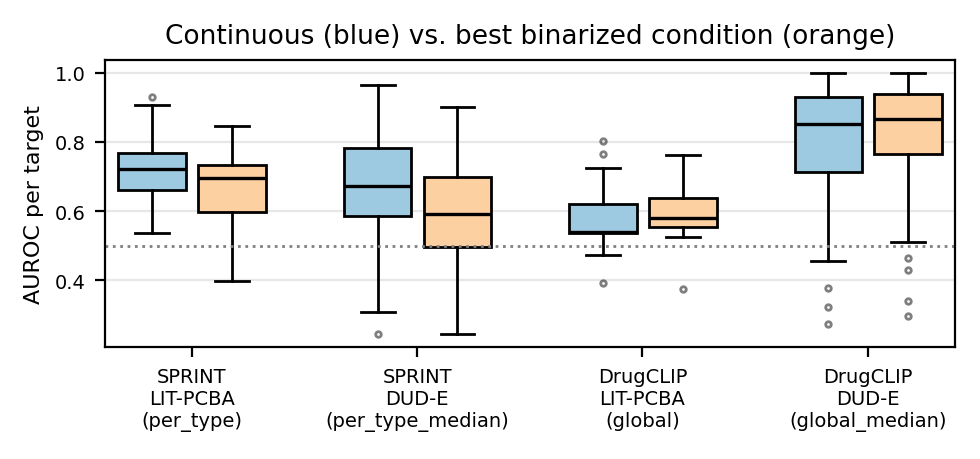
\includegraphics[width=10.8cm]{centering_sweep.png}
\caption{\label{fig:centering}Per-target AUROC: continuous cosine (blue) against the best binarized condition for
that model and benchmark (orange, named beneath each group). Boxes show the median and
interquartile range over targets, whiskers the range excluding outliers, circles the outliers.
The dotted line marks chance. The two models are mirror images of each other: for SPRINT the
binarized box sits below its continuous baseline on both benchmarks, whereas for DrugCLIP it
sits at or above it. Note also how wide the per-target spread is compared with the differences
between conditions.}
\end{figure}

\begin{table}[h]
\centering
\small
\caption{\label{tab:grid}Mean AUROC across all six scoring conditions. Bold marks the best binarized condition
per column. Each cell is a re-score of the same cached embeddings, so the conditions differ
only in the scoring function.}
\begin{tabular}{lrrrr}
\toprule
Condition & SPRINT & SPRINT & DrugCLIP & DrugCLIP \\
 & LIT-PCBA & DUD-E & LIT-PCBA & DUD-E \\
\midrule
cosine (continuous) & 0.7253 & 0.6759 & 0.5832 & 0.8071 \\
\midrule
Hamming, \texttt{none} & 0.5442 & 0.5285 & 0.5780 & 0.7918 \\
\texttt{per\_type} & \textbf{0.6662} & 0.5535 & 0.5547 & 0.7885 \\
\texttt{per\_type\_median} & 0.5201 & \textbf{0.5947} & 0.5407 & 0.7881 \\
\texttt{global} & 0.4274 & 0.3989 & \textbf{0.6006} & 0.8261 \\
\texttt{global\_median} & 0.3533 & 0.4201 & 0.5991 & \textbf{0.8280} \\
\bottomrule
\end{tabular}
\end{table}

The result worth emphasising is the \emph{direction}, not the size. Global centering beats
DrugCLIP's own continuous baseline by $+0.0190$ on DUD-E and $+0.0174$ on LIT-PCBA, which on
its own is a small gain and is smaller than the spread between the three published DrugCLIP
baselines. What makes it notable is that it is positive at all: compressing an embedding from
32 bits per dimension to 1 is expected to cost accuracy, and here it costs nothing. The same
operation applied to SPRINT gives 0.4274 and 0.3989, which is worse than random. One
preprocessing step therefore moves one model slightly up and the other far below chance,
which is a much stronger statement than either number alone.

Figure~\ref{fig:centering} also shows why the mean values should not be read too confidently. The per-target
AUROC spread on DUD-E runs from below 0.3 to 1.0, so a shift of 0.019 in the mean is small
against how much individual targets vary. The reason for trusting it is not its size but that
it replicates, with the same sign and magnitude, on a second benchmark.

\subsection{Why the two encoders differ}\label{sec:why-differ}
The two orderings are explained by the distributions of the embeddings themselves. For each
dimension of an encoder's output I computed where that dimension's mean falls within its own
values - at the 50th percentile the mean splits the dimension in half, and mean-centering then
produces a balanced bit.

DrugCLIP's distributions are close to symmetric, with the mean at the 49.9th percentile, so
mean-centering already produces a balanced code - a bit density (the fraction of bits set to
1) of 0.5008, with only 0.9\% of bits differing between mean and median centering. SPRINT's
are extremely heavy-tailed, with a skew of $+45.5$ and the mean at the 96.7th percentile, so
mean-centering produces a sparse code at a bit density of 0.033: a bit is set only for the
roughly 3\% of molecules with an unusually high value in that dimension. The median forces the
density to 0.500 and 46\% of bits differ. All of these were computed from the cached embedding
dumps, not taken from either paper.

Median centering is not a free improvement and for SPRINT on LIT-PCBA it is a large
regression, from 0.6662 to 0.5201. For an encoder with SPRINT's statistics the imbalance is
apparently carrying the signal, and forcing a balanced code destroys it.

\subsection{Post-hoc binarization against published metrics}\label{sec:posthoc}
Relative to its own continuous baseline, the best post-hoc condition improves global ranking
while degrading early enrichment. On DUD-E, global centering gives $+0.0190$ AUROC,
$-0.0272$ BEDROC and $-2.86$ EF 0.5\%.

\begin{table}[h]
\centering
\small
\caption{\label{tab:drughash}DrugCLIP on DUD-E, post-hoc binarization against DrugHash's published result. The
\texttt{none} row is the like-for-like match to DrugHash's $\lambda = 0$ ablation, since both
binarize without subtracting any reference.}
\begin{tabular}{lrrr}
\toprule
DUD-E & AUROC & BEDROC & EF 0.5\% \\
\midrule
cosine (continuous) & 0.8071 & 0.4733 & 36.46 \\
Hamming, \texttt{none} & 0.7918 & 0.4217 & 32.59 \\
Hamming, \texttt{global} & 0.8261 & 0.4461 & 33.60 \\
\midrule
DrugHash, published & 0.8373 & 0.5716 & 43.03 \\
\bottomrule
\end{tabular}
\end{table}

Against DrugHash's published row \citep{bib:drughash}, post-hoc binarization recovers 98.7\% of the AUROC but only
78.0\% of the BEDROC and 78.1\% of the EF 0.5\%. The \texttt{none} condition, which is the
setting DrugHash's ablation actually tested, loses on every column, at $-0.0153$ AUROC,
$-0.0516$ BEDROC and $-3.87$ EF 0.5\%, and therefore reproduces their finding.

This is what makes their claim an upper bound rather than a measurement of what hashing
contributes. DrugHash measures the value of its training by the gap between $\lambda = 0$ and
$\lambda = 0.2$, and attributes that whole gap to the hashing objective. But their
$\lambda = 0$ point binarizes without any centering, which Table~\ref{tab:drughash} shows is the worst of the
available post-hoc options. A single free preprocessing step recovers $0.0343$ AUROC of that
gap without any training at all. The part of their reported improvement that is genuinely
attributable to training is therefore smaller than the gap they report, and on AUROC
specifically it very nearly disappears. Their conclusion does survive for BEDROC and EF, where
even the best post-hoc condition remains well short of the trained result.

It should be noted that the $\lambda = 0$ values in DrugHash are plotted rather than tabulated
and no AUROC or BEDROC metrics are reported for the different $\lambda$ values in the
ablation. The comparison here therefore rests on their qualitative claim together with the
measured numbers in Table~\ref{tab:drughash}.

\subsection{Trained hash head}\label{sec:hash-head}
Applying DrugHash's objective to a head on frozen \emph{DrugCLIP} encoders, evaluated on
DUD-E, reverses the pattern of the previous section. Figure~\ref{fig:lambda} plots the sweep. Under plain $\operatorname{sign}(\cdot)$,
which is what the paper does, increasing $\lambda$ from 0 to 3 raises AUROC from 0.7853 to
0.8025, BEDROC from 0.4080 to 0.4655 and EF 0.5\% from 31.45 to 35.72. Expressed as relative
change, this is BEDROC $+14\%$, EF 0.5\% $+13.6\%$ and AUROC $+2.2\%$, so the gain is
concentrated in early recognition and not in global ranking.

\begin{figure}[h]
\centering
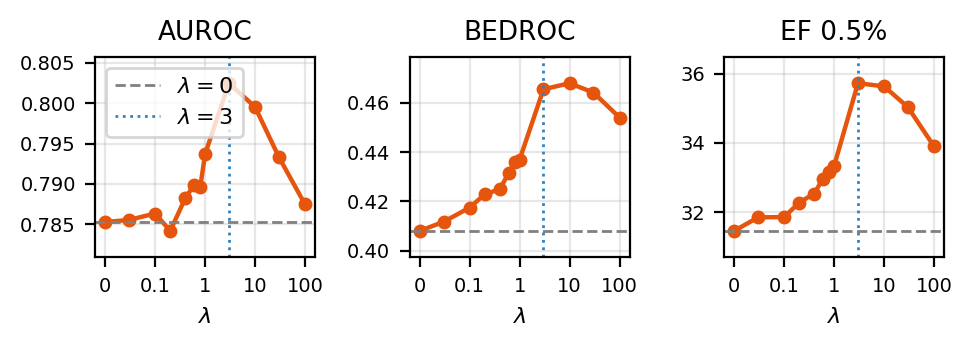
\includegraphics[width=10.8cm]{lambda_sweep.png}
\caption{\label{fig:lambda}Mean metrics over the 100 DUD-E targets for the trained hash head on frozen DrugCLIP
encoders, against the weight $\lambda$ on the hashing term. The dashed line marks the
$\lambda = 0$ baseline and the dotted line the optimum found here. All three metrics improve
together, but BEDROC and EF 0.5\% rise far more steeply than AUROC. Most of the movement
happens beyond $\lambda = 1$, which is where the paper's grid ends.}
\end{figure}

A mean over 100 targets can be produced by a few targets improving enormously while most get
worse, so the per-target results were also compared pairwise, matching each target's score at
$\lambda = 3$ against its own score at $\lambda = 0$. AUROC improves on 70 of 100 targets,
BEDROC on 69 and EF 0.5\% on 58, so the effect is broad rather than concentrated in a few
outliers.

The trained head also beats the best post-hoc condition from Table~\ref{tab:drughash}. Combining $\lambda = 3$
with global centering gives AUROC 0.8333, BEDROC 0.4774 and EF 0.5\% 36.34, against 0.8261,
0.4461 and 33.60 for global centering on its own, with BEDROC improving on 65 of 100 targets.

Set against each other the split is stark. Both routes improve AUROC by about two percent -
$+2.4\%$ for post-hoc centering and $+2.2\%$ for the trained head - but centering pays for it
with $-5.8\%$ BEDROC and $-7.9\%$ EF 0.5\%, where the trained head gains $+14.1\%$ and
$+13.6\%$ on those same two metrics.

Finally, the $\lambda$ grid the paper explores turns out to do almost nothing on a frozen
encoder. Across the whole range $\lambda \leq 1$, which is where the paper's grid ends, the
validation contrastive loss is flat to three decimal places and the gradient contributed by the
hashing term never exceeds 12\% of the gradient contributed by the contrastive term - the
hashing term is present in the loss but is too weak to change the solution. The optimum found
here is $\lambda \approx 3$ on AUROC and EF 0.5\%, with BEDROC peaking slightly later at
$\lambda = 10$; either way roughly 15 times the paper's 0.2. This is expected rather than a
contradiction: DrugHash can use a small $\lambda$ because its encoders are also being updated
and can move a long way over training, whereas here only a single linear layer can move, so a
much larger weight is needed before the hashing term influences the result at all. The
practical consequence is that any $\lambda$ sweep on a frozen encoder has to extend past the
published grid, otherwise the flat curve would be misread as evidence that hashing does
nothing.

\subsection{Code length and a tie-breaking artefact}\label{sec:code-length}
Truncating SPRINT's code initially appeared to improve accuracy. LIT-PCBA AUROC rose from
0.6662 to 0.7152 at 64 bits and EF 0.5\% from 4.40 to 6.83, monotone in code length and
replicating across DUD-E's 102 targets, which would have been a 16x memory reduction with an
accuracy gain.

Table~\ref{tab:truncation} gives the result that survives a fair tie-break; the initial one was
entirely an artefact of tie-breaking. Table~\ref{tab:truncation} is the only table in this
report scored that way: every other table and both figures use the default actives-first
policy, so the hashed numbers in them should be read as upper bounds. A $k$-bit code admits at most $k+1$ distinct
Hamming similarities, so ties are the norm rather than the exception. The sort used was stable,
meaning tied entries keep their original order, and the molecules are loaded actives-first,
which means every tie resolved in favour of the actives. Shortening the code multiplies the
number of ties, which is exactly why the effect looked cleanly monotone in code length. On
MAPK1, one of the 15 LIT-PCBA targets, AUROC falls from 0.7264 to 0.6503 and EF 0.5\% from
8.82 to 3.15 once ties are broken at random instead.

\begin{table}[h]
\centering
\small
\caption{\label{tab:truncation}SPRINT under truncation with a seeded random tie-break, so that tied molecules are
ordered randomly rather than actives-first.}
\begin{tabular}{lrrrr}
\toprule
 & \multicolumn{2}{c}{LIT-PCBA} & \multicolumn{2}{c}{DUD-E} \\
\cmidrule(lr){2-3}\cmidrule(lr){4-5}
Bits & AUROC & EF 0.5\% & AUROC & EF 0.5\% \\
\midrule
1024 (native) & 0.6606 & 4.15 & 0.5477 & 1.89 \\
512 & 0.6527 & 3.47 & 0.5437 & 1.73 \\
256 & 0.6483 & 3.89 & 0.5423 & 2.02 \\
128 & 0.6417 & 2.81 & 0.5534 & 1.96 \\
64 & 0.6460 & 2.70 & 0.5472 & 2.01 \\
\bottomrule
\end{tabular}
\end{table}

With fair tie-breaking the surviving result is less dramatic but more useful. SPRINT tolerates
a 16x shorter code at a cost of 0.0146 AUROC on LIT-PCBA and 0.0005 on DUD-E, going from 1024
to 64 bits. Nothing is won by shortening, but almost nothing is lost either. Variance-ranked
dimension selection is catastrophic at 0.3883, since the highest-variance dimensions of a
heavy-tailed embedding are dominated by a few extreme values and binarize to near-constant
bits.

\subsection{Training-set leakage}\label{sec:leakage}
A benchmark active that the model was trained on is being remembered rather than retrieved, so
it is worth knowing how many there are. The molecules the released DrugCLIP checkpoint was
trained on are published alongside it, so I canonicalised the SMILES strings on both sides with
RDKit \citep{bib:rdkit} and
counted how many benchmark actives appear in that training set. Table~\ref{tab:leakage} gives
the counts.

\begin{table}[h]
\centering
\small
\caption{\label{tab:leakage}Benchmark actives that also appear in the released DrugCLIP checkpoint's training
ligands.}
\begin{tabular}{lrrr}
\toprule
Benchmark & Actives & Also in training & Targets affected \\
\midrule
DUD-E & 22{,}805 & 583 (2.56\%) & 90 / 102 \\
LIT-PCBA & 9{,}954 & 36 (0.36\%) & 10 / 15 \\
\bottomrule
\end{tabular}
\end{table}

DUD-E's exposure is roughly seven times higher than LIT-PCBA's. This applies equally to
DrugCLIP's own published numbers, since it is the same training set, so it is a property of
the benchmark and checkpoint pair rather than of this reproduction.

Leakage on the protein side was not checked, and importantly this is not the same as finding
none. DUD-E names its pockets by its own target codes, such as \texttt{aa2ar}, while
DrugCLIP's training pockets are named by PDB identifier, such as \texttt{10gs}. Intersecting
the two lists returns zero simply because the two naming systems share no strings at all, not
because the pockets are different. Establishing whether there is overlap would require mapping
DUD-E targets to PDB entries, which was not available offline.

\section{Discussion}\label{sec:discussion}

\subsection{Interpretation}

The two encoders differ not in how well they binarize but in what binarization does to them.
SPRINT's heavy tails mean that mean-centering produces a sparse and selective code, in which
the imbalance itself carries the signal. DrugCLIP's near symmetric dimensions mean that a 
shared origin is precisely what its two encoders were aligned on during contrastive training, 
which is why removing it hurts the performance and why sharing one helps.

Global centering weakens SPRINT because the shared reference is computed over the 
concatenation of the drug and target matrices and drugs outnumber targets by four to five
orders of magnitude. The shared reference is therefore effectively the drug mean and the 
target codes end up thresholded against the wrong distribution.

The reproduction asymmetry in Section~\ref{sec:repro} is informative as well. DrugCLIP trains a
separate model per benchmark but releases only one checkpoint, whose described training data 
matches the DUD-E recipe rather than the LIT-PCBA one. The closer DUD-E reproduction is 
consistent with that and if LIT-PCBA targets were present in the checkpoint's training data 
the bias would be upward, which is the direction the +0.0115 delta actually points. 
This is an inference from the paper and repository rather than something confirmed against 
the training data.

DrugHash's own reported gain over DrugCLIP has the same shape as the trained head's, so two
independent routes agree: binarizing a finished encoder improves the global ranking, and
training improves the top of the list.

\subsection{Limitations}\label{sec:limitations}

Several features of this setup constrain how the numbers above can be interpreted.

First, the trained head is a lower bound rather than a reproduction. The encoders are frozen 
and cannot adapt to being binarized and that adaptation is most of what DrugHash does, so the 
real method should outperform Section~\ref{sec:posthoc}.

Second, 2.56\% of DUD-E actives are present in the checkpoint's training ligands, which means 
absolute DUD-E values partly measure memorisation rather than retrieval. This applies equally 
to the published metrics, but it does mean the deltas between conditions are more trustworthy
than the absolute values, because they share that exposure.

Third, $\lambda \approx 3$ was identified by looking at the benchmark. The inner-validation 
objective contains $\lambda \cdot L_{\text{hash}}$ and is therefore not comparable across $\lambda$, 
so it cannot select it. The full curve is reported rather than a single chosen point and the 
curve is smooth rather than a spike, but the statement that $\lambda \approx 3$ is best remains 
an observation on DUD-E and not a held-out result.

Fourth, the centering effect is of the same order as the reproduction spread. The $+0.0190$ 
gain on DUD-E sits against a 0.0148 spread across the three available DrugCLIP baselines. The 
reason to believe the effect is that it replicates on LIT-PCBA with the same sign and magnitude, 
not the DUD-E measurement on its own.

Fifth, hashed enrichment factors are tie-dominated. A 128-bit code admits at most 129 distinct
similarity values and only 30 to 76 are observed per target, so the top 0.5\% of a library of 
several hundred thousand molecules is frequently a single tie block. Hashed AUROC should be treated 
as meaningful and hashed EF as indicative at best. Those ties are also broken in a direction
that favours the result: molecules load actives-first and the sort is stable, so every tie in a
hashed condition resolves towards an active, while the continuous baseline is effectively
tie-free. Section~\ref{sec:code-length} shows this was worth 0.0056 AUROC on one SPRINT
condition, and the hashed-versus-continuous gaps reported here are not separated from it. 

Beyond these, no hash head was trained for SPRINT at all, so the trained-route result rests on
a single encoder and the claim that the two routes behave differently is only demonstrated on
DrugCLIP. No DTI checkpoint was ever published for SPRINT, so that half of its paper cannot be 
reproduced, a zero-shot run on BIOSNAP reaches AUPR 0.574 against the 0.858 published for the
same 16M model, which is expected
rather than a failure. Additionally, nothing here runs at billion scale and Hamming scoring was 
computed densely rather than through an index, so this work measures accuracy under compression and not 
retrieval speed.

\subsection{Relation to the literature and broader implications}

The upper-bound argument of Section~\ref{sec:posthoc} is the sharpest point this work has to make about
the literature, and it is worth being precise about what it overturns. DrugHash's conclusion
really has two parts: that hashing must be trained in to preserve global ranking, and that it
must be trained in to preserve early recognition. Centering overturns the first and leaves the
second standing.

The transfer implication is the broader one. The effect of binarization depends on the geometry of the 
embedding space rather than on the hashing method alone, which means a scheme developed on DrugCLIP should 
not be assumed to work on SPRINT. Since DrugHash is developed on DrugCLIP, this is not a hypothetical concern.

For future work, two consequences follow. A trained hashing objective should be judged on BEDROC and EF 
rather than on AUROC, since AUROC is already saturated by a free post-hoc step. And SPRINT's tolerance of 
a 16x shorter code sets the memory budget such a method would have to work within.

\section{Conclusion}\label{sec:conclusion}

Two structure-aware screening models were reproduced within one to two points of their published
AUROC, DrugCLIP's DUD-E BEDROC 3.2 points low, and 
the cost of binarizing their embeddings was then measured on both.

The two encoders respond to binarization in opposite directions, across 117 SPRINT and 115
DrugCLIP targets on two benchmarks, and the mechanism is visible in their per-dimension statistics rather than in the scoring method. 
A hashing scheme tuned on one of them should therefore not be assumed to transfer to the other. 

Post-hoc binarization and a trained objective preserve different halves of the ranking. Centering a frozen encoder's 
codes preserves and slightly improves global ranking quality, whereas a trained objective improves early recognition 
and two independent routes agree on that observation. The practical consequence is that a hashing objective
should be judged on BEDROC and EF rather than on AUROC, which a free post-hoc step already
saturates. 

The work reported here is an initial exploration rather than a complete evaluation. The trained head runs on frozen 
encoders and is a lower bound, $\lambda$ was selected on the benchmark and a measurable fraction of the DUD-E actives 
were seen during the checkpoint's training. What the results do establish is that the interesting question is not 
whether binarization works, but which part of the ranking it preserves and that the answer depends on the encoder as 
much as on the method.

{\small
\setlength{\bibsep}{0.3ex}
\bibliographystyle{plainnat}
\bibliography{references}
}

\end{document}
